\documentclass[12pt,a4paper]{article}
\usepackage{titlesec}
\usepackage{fancyhdr}
\usepackage{titlesec}
\newcommand{\sectionbreak}{\clearpage}
\usepackage{apacite}
% !TEX TS-program = pdflatex
% !TEX encoding = UTF-8 Unicode
\usepackage[utf8]{inputenc} % set input encoding (not needed with XeLaTeX)
\usepackage{graphicx} % support the \includegraphics command and options
\usepackage{pdfpages}

%%% PACKAGES
\usepackage{booktabs} % for much better looking tables
\usepackage{array} % for better arrays (eg matrices) in maths
\usepackage{paralist} % very flexible & customisable lists (eg. enumerate/itemize, etc.)
\usepackage{verbatim} % adds environment for commenting out blocks of text & for better verbatim
\usepackage{subfig} % make it possible to include more than one captioned figure/table in a single float
\usepackage[toc,page]{appendix}
\usepackage{url}

\makeatletter
\renewcommand\paragraph{%
    \@startsection{paragraph}{4}{0mm}%
       {-\baselineskip}%
       {.2\baselineskip}%
       {\normalfont\normalsize\bfseries}}
\makeatother

\hbadness=99999

%header and footer settings
\pagestyle{fancyplain}
\fancyhf{}
\renewcommand{\headrulewidth}{0.5pt}
\renewcommand{\footrulewidth}{0.5pt}
\setlength{\headheight}{15pt}
\fancyhead[L]{Jacob Barrow - 40337360}
\fancyhead[R]{ SOC10101 Honors Project}
\fancyfoot[L]{}
\fancyfoot[C]{\thepage}


\usepackage{listings}
\usepackage{xcolor}

\definecolor{codegreen}{rgb}{0,0.6,0}
\definecolor{codegray}{rgb}{0.5,0.5,0.5}
\definecolor{codepurple}{rgb}{0.58,0,0.82}
\definecolor{backcolour}{rgb}{0.95,0.95,0.92}

\lstdefinestyle{mystyle}{
    backgroundcolor=\color{backcolour},   
    commentstyle=\color{codegreen},
    keywordstyle=\color{magenta},
    numberstyle=\tiny\color{codegray},
    stringstyle=\color{codepurple},
    basicstyle=\ttfamily\footnotesize,
    breakatwhitespace=false,         
    breaklines=true,                 
    captionpos=b,                    
    keepspaces=true,                 
    numbers=left,                    
    numbersep=5pt,                  
    showspaces=false,                
    showstringspaces=false,
    showtabs=false,                  
    tabsize=2
}

\lstset{style=mystyle}


\newif\iffluff

\flufffalse

%this starts the document
\begin{document}

\newcommand{\HRule}{\rule{\linewidth}{0.5mm}}

\begin{titlepage}
	\begin{center}

	\HRule \\[0.4cm]
    	{\Large \bfseries Detecting Incongruous News Articles \par}
	\vspace{0.2cm}
	\HRule \\[1.5cm]

	
    	\vspace{3cm}
	\begin{minipage}{0.4\textwidth}
	\begin{center} \large
        \emph{}\\
        	Jacob Barrow - 40337360
				
   	 \end{center}
    	\end{minipage}
	
	\vspace{2cm}
    	\begin{minipage}{1\textwidth}
    	\begin{center} \large
        
		Submitted in partial fulfilment of\\
		the requirements of Edinburgh Napier University\\
		for the Degree of\\
        	BSc (Hons) Computing Science
    	\end{center}
    	\end{minipage}

    	\vfill

    	% Bottom of the page
	\begin{minipage}{1\textwidth}
    	\begin{center} \large
		School of Computing
    	\end{center}
    	\end{minipage}
	
	\vspace{1cm}
    	{\large \today}


	\end{center}
\end{titlepage}
%{\large Submitted in partial fulfilment of the requirements of Edinburgh Napier University for the Degree of }
\iffluff

\section*{Authorship Declaration}
\vspace{0.5cm}
\begin{flushleft}
I, Jacob Barrow, confirm that this dissertation and the work presented in it are my own achievement.\newline

Where I have consulted the published work of others this is always clearly attributed;\newline

Where I have quoted from the work of others the source is always given. With the exception of such quotations this dissertation is entirely my own work;\newline

I have acknowledged all main sources of help; \newline

If my research follows on from previous work or is part of a larger collaborative research project I have made clear exactly what was done by others and what I have contributed myself;\newline

I have read and understand the penalties associated with Academic Misconduct.\newline

I also confirm that I have obtained informed consent from all people I have involved in the work in this dissertation following the School's ethical guidelines.\newline
\end{flushleft}

\begin{flushleft} \large
\emph{Signed:} \\
\end{flushleft}

\includegraphics[height=1cm]{images/sig.png}


\begin{flushleft} \large
\emph{Date:} 19/04/2021 \\
\end{flushleft}

\vspace{.5cm}

\begin{flushleft} \large
\emph{Matriculation no: } 40337360  \\
\end{flushleft}

\pagebreak

\section*{General Data Protection Regulation Declaration}
\vspace{0.5cm}
\begin{flushleft}
Under the General Data Protection Regulation (GDPR) (EU) 2016/679, the University cannot disclose your grade to an unauthorised person. However, other students benefit from studying dissertations that have their grades attached. \newline

\vspace{0.5cm}

Please sign your name below one of the options below to state your preference.\newline
\vspace{0.5cm}

The University may make this dissertation, with indicative grade, available to others.\newline
\vspace{3cm}


The University may make this dissertation available to others, but the grade may not be disclosed.\newline
\vspace{3cm}


The University may not make this dissertation available to others.\newline
\end{flushleft}



\pagebreak
\fi

\begin{abstract}
% fill the abstract in here
\end{abstract}
\pagebreak

\tableofcontents % is generated for you
\newpage

\iffluff
\listoftables
\newpage

\listoffigures
%you may have captions such as equations, listings etc they should all appear as required
%these are done for you as long as you use \begin{figure}[placement settings] .. bla bla ... \end{figure}
\newpage

\section*{Acknowledgements}
Insert acknowledgements here
\newpage
\fi

\section{Introduction}
Fake news, disinformation and misleading articles have been the subject of much debate and controversy. With the decline of traditional print media, more people turn to online sources for news, where publishing has a much lower barrier to entry.

Incongruous headlines misrepresent the content of an article and, intentional or not, can lead to the formation of unfounded opinions and misconstrued facts. To combat this, existing articles should be analysed to ascertain the extent of the problem, and a system created whereby the congruence of new articles can be determined.

Considering the rate at which publishers output news articles, it would be impractical for a human-scale operation to undertake this task. Therefore, this dissertation seeks to create a classifier capable of calculating a measure of a headline's incongruence, by utilising Natural Language Processing (NLP) to analyze the components of a news article.

As the laws of natural language - the spoken and written means by which humans communicate with each other - are uncodified, blurry and change from generation to generation, analysing the meaning of text poses a considerable challenge.  For instance, while the sentiment of a headline may be completely at odds with an article's content, this could potentially be a sarcastic or ironic technique used by the publisher.

Overcoming these obstacles requires a thorough understanding of NLP, and the range of approaches and techniques used to identify and extract meaning from text.

A considerable set of articles will need to be created, with both a longitudinal aspect spanning a large period of time, and a cross-section of the current state of online news articles. Additionally, to provide both a baseline and a method of training a classifier, a portion of this dataset will need to be labelled with absolute values of congruence.


\subsection{Aims}
The primary aim of this dissertation is to create an incongruence classifier. Additionally, a large dataset of news articles will be created and a subsection of them labelled.

\subsection{Research Questions}
In order to judge the success of the project, and to provide a direction for research, this dissertation seeks to answer the following questions:
\begin{itemize}
	\item To what extent do incongruent articles exist in current contemporary online news?
	\item How, if at all, has the congruence of news articles changed over the decade?
	\item How effective is NLP in determining the congruence of a news article's headline?
\end{itemize}

\subsection{Project Outline}
The project will consist of a range of deliverables and milestones.
 
\paragraph{Background Research}
A literature review will be undertaken to provide context to the project and define its scope

\paragraph{Data collection}
In order to provide the algorithm with articles to classify, a dataset is required. It will be sourced from a range of publishers, and idealy cover a large timescale to allow trends to be identified.

\paragraph{Data Labelling}
A raw dataset can be made more valuable by creating a training set from it. This will be a small subsection of the articles that volunteers will label with their perception of the incongruence.

\paragraph{Algorithm Creation}
Once a dataset is generated and labelled, the algorithm to classify the articles can be implemented. 

\paragraph{Analysis}
The algorithm will create a range of data points that can be analysed. Trends will be spotted in the dataset used, and comparisons made with different implementations of the algorithm.

\pagebreak
\section{Background Research}
\subsection{Introduction}
This study aims to create a method of detecting incongrouence in news articles. Before the implementation begins, it's important to review the existing literature to give the study context.

First, this research begins by defining different types of incongruence and specifying the bounds of incongruence applicable to this study. 

Several existing approaches are then evaluated and discussed to give a clearer picture of both what's already been done, but also to gain some insight into a possible approach to tackle the problem.

Then, natural language processing (NLP) is defined and different features and approaches reviewed and discussed.

\subsection{Types of Incongruence}
Incongruence is a broad term that, when applied to news media, covers a lot of different forms of deception and misleading information. \citeA{chesney2017} classifies three different types of incongruent news articles: clickbait, fake news, and sensationalism.

\paragraph{Clickbait}
\citeA{potthast2016} define clickbait as a kind of "web content [...] designed to entice its readers into clicking an accompanying link". Clickbait uses exaggerated language, outright fake information and can be accompanied by graphics designed to entice a reader. Figure \ref{fig:clickbait} shows an example of clickbait, sourced from a Natural Health website \footnote{\url{https://naturalon.com/}}.

\begin{figure}[ht!]
  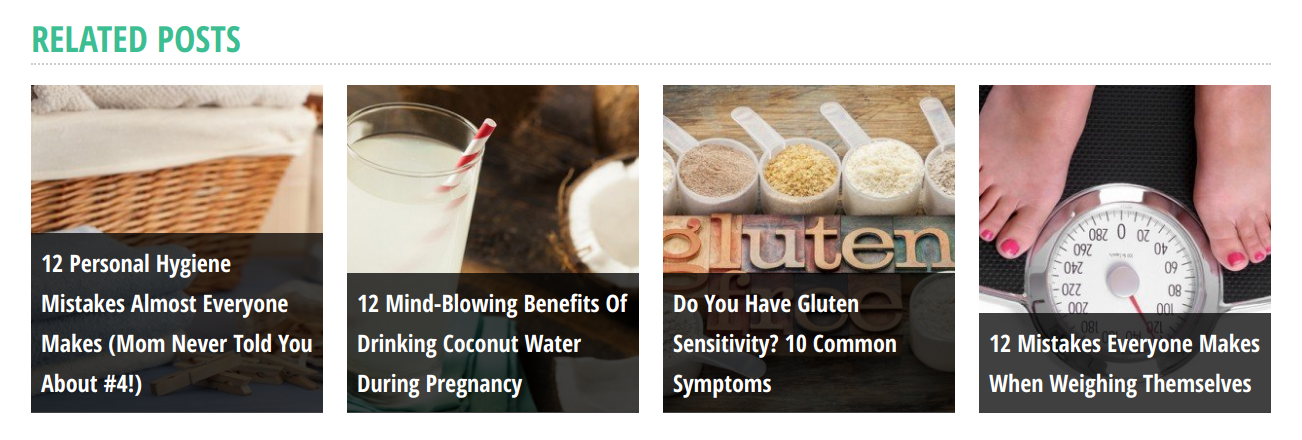
\includegraphics[width=\linewidth]{images/clickbait.png}
  \caption{Several clickbait articles in a 'chum box'}
  \label{fig:clickbait}
\end{figure}

\citeA{mahoney2015} terms a collection of clickbait stories as a 'chum boxes' - chum being dead fish used as bait for other fish. \citeauthor{mahoney2015} goes on to examine how clickbait uses psychological methods to manipulate, and how they can have an unconscious effect on an individual.

\paragraph{Fake News}
\citeA{allcott2017} defines fake news to be "news articles that are intentionally and verifiably false, and could mislead readers". For example, a fake news conspiracy theory claimed that a pizzeria, Comet Ping Pong, in Washington ran a child sex ring in its basement. Figure \ref{fig:fakenews} shows a news article from 2016 from Your News Wire\footnote{\url{https://archive.is/YTk3n}} (now News Punch).


\begin{figure}[ht!]
  
\includegraphics[width=\linewidth]{images/fakenews.png}
  \caption{A fake news story}
  \label{fig:fakenews}
\end{figure}


This lead to a man walking into Comet Ping Pong with an assault rifle and firing several shots. The restaurant's owner and staff also received several death threats \cite{lopez2016}. 

\citeauthor{allcott2017} go further in their definition, and give the following sub-categories for fake news: satire, parody, fabrication, manipulation, advertising and propaganda. While the intention of satire and parody is not to deceive but to criticise, the other classifications have more subversive aims, such as misinforming people or gaining as many clicks as possible.

\paragraph{Sensationalism}
\citeA{molek2013} defines sensationalism as "a specific discourse strategy  aimed  at  channeling  audience's  attention,  which  may  well  be  resorted  to  by  both  popular and quality outlet". They suggest that media fails to provide important and valuable news, in preference for that which is superficial and quick-paced.


Below are examples of sensationalised headlines, sourced from The Sun:

\begin{itemize}
	\item DOOMSDAY DISEASE FEARS Terrorists could turn ‘sniff and die’ virus that kills victims in 24 hours into a BIO-WEAPON
	\item SPICE UP YOUR LIFE Chilli and ginger ‘slash the risk of cancer – stopping tumours growing’
	\item JAB DEBATE As Melinda Messenger slams the HPV jab the parents of two teenagers blame their daughters’ ‘paralysis on vaccine’
	\item 'I KNOW WHO KILLED JONBENET' Juror from the JonBenet Ramsey case gives sensational interview revealing he ‘knows who killed six-year-old’
	
\end{itemize}

These headlines use dramatic language ('slams', 'sensational', 'slash') to evoke a sense of urgency and excitement in the reader, urging them to click through to the rest of the article. Unlike clickbait headlines, information is not withheld but rather dramatised - while the aim is still to get as many clicks as possible, this is achieved through different means.

This sensationalism is intended to provoke and entertain, at times at the expense of accuracy \cite{chesney2017}.

\subsubsection{Project scope}
This project will not consider fake news - by its nature, the entirety of a fake news article will be false, not just the headline. Therefore, to determine whether an article is fake, external sources would have to be consulted. Creating an algorithm for the truth, while an open problem in computer science\footnote{\url{https://www.youtube.com/watch?v=leX541Dr2rU}}, is considered out of the scope of this project.

Instead, this study will seek to evaluate to what extent a headline represents an article's body. This could identify sensationalism, over-exaggerated news stories and potentially some types of clickbait.

\subsection{Impact of Incongruence}
\citeA{karlsson2010} categorise online news both by its immediacy and interactivity, which has shortened the news cycle and increased the competitivity between publishers. Therefore, publishers have to make the news more appealing to potential consumers.

In the information-overload arena of online news reporting, the body of a news article is less read than the headline \cite{gabielkov2016}.  

For those that read beyond the headlines, incongruent articles can still be problematic; it's a well-established theory in psychology that first opinions matter \cite{digirolamo1997}. \citeA{ecker2014} ran a study that investigated how headlines affect the processing of the facts in news "Information that is initially accepted as valid but is later found to be incorrect can have a persistent influence on people’s memory and reasoning". Publishers can seek to sway individuals by using choice phrases to influence their mindset, which means that the same content could be interpreted in many ways depending on its headline \cite{reis2015}.

This means that if a headline is incongruent, even if the individual reads the whole article, there's a real possibility they will be left with a false impression of the facts. 


\subsection{Existing Approaches} \label{existing-approaches}

\citeA{manjesh2017} used a range of different techniques to identify clickbait and were able to achieve a 98\% accuracy with a deep learning approach. However, they only analysed the article's headline and disregarded the body text.  They found that clickbait headlines tend to have elaborate sentences with various linguistic nuances, such as "21 Pics Of Celebs Photoshopped In The Best Way Ever. These Are EPIC". There's also a statement at the end to further strengthen the main claim of the headline.

\citeA{park2020} used a deep learning approach to create a web interface for detecting incongruent articles. They managed to gain an accuracy of 86\%. However, for their dataset, they generated incongruent articles by swapping a completely different article's text in for the original. For example Headline A would have a section of Article B's body. They then considered congruent headlines to be those with the original body text in place. This could lead to false positives, and as the manufactured dataset does not reflect the incongruence in real-world articles their algorithm's output lacks validity.

The first Fake News Challenge (FNC1) was held by \citeA{pomerleaurao2017}. The challenge supplied a dataset of articles, and encouraged contestants to create a classifier capable of detecting fake news. While there has not been subsequent challenges, 50 teams competed and produced a wide range of different approaches. 

\subsubsection{Exisiting Labelled Datasets}
A labelled dataset is a set of data points that have been tagged with some information that identifies a characterstic of that data. For example, for this project a labelled dataset may consist of several articles that have been tagged with a level of congruence. Labelled datasets can be used to inform and train an algorithm to correctly tag unlabelled data, or be used as a 'gold-standard' to determine the performance of a system.

\citeA{chesney2017} reviews the current datasets available to detect incongruent articles, and concludes that while many are available and have some potential use, none are a good fit for the task.

\begin{table}[h]
\begin{tabular}{p{4cm}p{7.5cm}l}
\textbf{Source} & \textbf{Labels} & \textbf{Size} \\
Clickbait Challenge & Discrete (Not\-/Slightly\-/Considerably\-/Heavily Clickbaiting) & 2495 \\
\citeA{piotrkowicz2017} & Continuous (prominence, sentiment, superlativeness, proximity, surprise, and uniqueness) & 11980 \\
FakeNews Challenge & Discrete (Agree, Disagree, Discuss, Unrelated) & 50000 \\
\end{tabular}
\caption{An overview of existing labelled datasets}
\label{tab:existing-data}
\end{table}

\subsection{Natural Language Processing}
Natural language processing (NLP) is a method of extracting information from a spoken or written language. 'Natural' here means the more free and less well defined human language, as opposed to strictly interpreted programming and mathematical notation. \cite{jackson2002}

 As natural language is filled with a range of nuances, assumptions and relies heavily on context, codifying it into a standardised, programmatic output poses a range of difficulties. For example, consider the following two sentences:

\begin{itemize}
	\item Apple's shares fell by 10\% in the last quarter
	\item An apple a day keeps the doctor away
\end{itemize}

The word 'apple' appear in both sentences, but in one it refers to a multinational company, and in the other a tasty fruit. It is only by using the context clues in the surrounding sentence that the meaning of the word can be deduced.

There are a range of different approaches that seek to tackle the problems inherent in determining the meaning and sentiment of natural language, each with their  characteristics, strengths and limitations. 

\subsubsection{Statistical NLP}
Statistical NLP creates metadata from a sentence and aims to extract meaning by using statistical inference \cite{manning1999}. Several techniques can be used to create and interpret the metadata.

\paragraph{Tokens}
A token is typically an alphanumeric string or a punctuation mark. For instance, the sentence "Is this the way to Amarillo?" could be tokenised (represented as a list of tokens) like so: \texttt{"Is", "this", "the", "way", "to", "Amarillo", "?"}.\par
	
\paragraph{n-grams}
An n-gram is a subsection of a tokenised sentence, where \texttt{n} represents the number of tokens in a subsection. An n-gram of length 3 (also known as a tri-gram) of the above sentence could be \texttt{"way", "to", "Amarillo"}
	The location of these n-grams, their frequency and their composure all provide data points that can provide insights into the meaning of a body of text \cite{banerjee2003}.
	
\paragraph{Colocations}
\citeauthor{manning1999} describe a colocation as "an expression consisting of two or more words that correspond to some conventional way of saying things". For example, "around about", "stark naked" and "stiff upper lip" are all colocations. In a colocation, the subsequent parts make up a whole and lose some of their independent meaning - "fool hearted" makes sense to an English speaker's ear, but "idiot hearted" could sound offensive, or cause a misunderstanding.
	One way of identifying colocations is to count the frequency of bigrams in a body of text - a high number of two words occurring next to each other could indicate a colocation. \\

By themselves, these techniques would be insufficient to extract any substantative meaning or measure of congruence from an article. However, they will be essential in the formation of a foundation for a classifier, and knowledge of them will be crucial in understanding the more advanced and complex NLP approaches.

\subsubsection{Sentiment Analysis}\label{lit:sentiment-analysis}
Sentiment analysis is a branch of NLP that could potentially aid the detection of an incongrous article. It's a relatively new development (no substantial research had been conducted before 2000) that aims to extract opinions from text and speech \cite{liu2012}.

\citeA{liu2012} identifies a key problem with sentiment analysis: sentiment is a very subjective concept, and calculating an absolute sentiment score for a sentence is fraught with potential difficulties. For instance, the phrase "I really enjoy writing in an academic style" could be interpreted as a very positive remark, or perceived with sarcastic overtones and classified as a negative sentiment.

Sentiment analysis could be used to approach this project - both the headline and the body could be analyised, and the results compared. The difference in sentiment could then be used as an incongruence score.

However, it is possible for two pieces of text to share the same sentiment, yet disagree with eachother. For instance, consider the following two phrases:

\begin{itemize}
	\item I love Daniel Craig's work - he's the best Bond
	\item Sean Connery is by far the best Bond, he's a great actor
\end{itemize}

While both have a very positive sentiment regarding each actor's ability, they are completely opposed in opinion. Likewise, it's also possible for two texts to have opposing sentiments and yet be congruent in meaning - a headline could  be a positive sentiment about wind turbines, yet the body could contain very negative sentiments about coal-fuelled power plants.

Because of these issues, sentiment analysis by itself would not provide a significant metric by which the congruence of an article can be determined. However, it could prove beneficial to integrate it alongside other NLP techniques. 

\subsubsection{Named Entity Recognition}
Named Entity Recognition (NER) is the process of extracting and locating references to real-world objects from text. These named entities can represent a wide number of 'information units', such as people, organisations, locations and numeric expressions \cite{nadeau2007}. 

There are several approaches to NER, two of which are covered here.

\paragraph{One Hot Encoding}
One hot encoding represents each word in a phrase as a binary string, with the length of the string being the number of unique tokens in the phrase \cite{bommana2019}.  For example, consider the following sentence "I've got to go to France!", which can be tokenised as:
\begin{center}\texttt{"I've", "got", "to", "go", "to", "France", "!"}
\end{center}

\begin{minipage}{0.25\textwidth}
\begin{tabular}{ll}
I've   & \texttt{100000} \\
got	   & \texttt{010000} \\
to	   & \texttt{001000} \\  
go 	   & \texttt{000100} \\  
France & \texttt{000010} \\  
!	   & \texttt{000001} \\  
\end{tabular}
\end{minipage}
\begin{minipage}{0.68\textwidth}
This can be encoded using the one hot method, using a binary string of length 7, as on the left.

These binary representations can then be consumed by a neural network, which can be trained to identify named entities by detecting patterns in the makeup of the encoded strings.

\end{minipage}

\paragraph{Word Vectorisation}\label{lit:word2vec}

The act of converting a word to a vector (word2vec) is a simple but powerful concept. As well as being used to identify words with similar meanings, it can also identify analgous pairs and connections between words. The most famous of these analogies is "Man is to king as woman is to \textit{x}", where word2vec is able to give \textit{x} as "queen". \cite{church2017}


\begin{minipage}{1.5in}

\end{minipage}

\begin{minipage}{0.4\textwidth}
\begin{center}
\framebox{\textbf{I've} got to} go to France!\\ \vspace{1mm}
\framebox{I've \textbf{got} to go} to France!\\ \vspace{1mm}
\framebox{I've got \textbf{to} go to} France!\\ \vspace{1mm}
I've \framebox{got to \textbf{go} to France}!\\ \vspace{1mm}
I've got \framebox{to go \textbf{to} France!}\\ \vspace{1mm}
I've got to \framebox{go to \textbf{France}!}\\ \vspace{1mm}
I've got to go \framebox{to France\textbf{!}}\\ 
\end{center}
\captionof{figure}{Context windows}\label{fig:context-window}

\end{minipage}
\begin{minipage}{0.5\textwidth}
These core concept of these connections are 'context windows' - a set of words that surround a target. For instance, using a window of size 2 (2 tokens on either side of the target), the example sentence would be analyised as in figure \ref{fig:context-window} (the target token is emboldened).\\
Bigrams (pairs of tokens) can then be taken for each window, and the collection of bigrams then used to train a neural network to generate a vector.
\end{minipage}

\vspace{2mm}

These vectors take the form of an array of floats used to represent a word - for instance, "cat" could be represented as \texttt{[0.023, 0.131, 0.001, 0.415, 0.901]}. The length of the array is determined by the number of neurons in the hidden layer of the neural network, as each neuron is responsible for calculating a single float \cite{bommana2019}. These vectors can be thought of a point in a multi-dimensional space, and connections can be made by traversing the dimensions to find new words.

In terms of the scope of this project, word vectorisation could provide some useful insight into the relatedness of the headline and the body text. Again, this may not be sufficient as a standalone technique, but when used as part of a larger pipeline, it has potential to yield some good results.

\subsubsection{Lexical Overlap}
Lexical overlap, also known as lexical similiarty or textual entailment, is a measure of similarity between two elements of text \cite{adams2006}. This overlap can either be character-based (similar text) or statement-based (similar meaning).

\citeA{pradhan2015} reviewed several different approaches to obtaining a measure of lexical overlap. Statement-based lexical overlap uses the distance between word vectors to determine the difference in sentiment. Cosine similarity can be used to calculate the distance between two words by taking into account the angle created between the vectors and the origin \cite{qian2004}. Alternatively, the difference between a single word and a set of words can be calculated using centroid-based similarity. This is the measure of distance from one point in a vector to the geometrical centre (the arithmetic mean) of a set of points \cite{Awrejcewicz2012}.  

Character-based lexical overlap is used to determine how similar words are in respect to their composition. For example, 'witches' has a large character overlap with 'britches', but very little overlap with 'broomstick'. The Levenshtein distance can be used to calculate overlap, and is loosely defined as 'the minimum number of [operations] to make two strings equal' \cite{navarro2001guided}. Other distance measures include the Hamming distance (number of replacements), the Episode distance (number of additions) and the Longest Common Subsequence distance (number of additions and deletions). 



\subsubsection{tf-idf}\label{lit:tfidf}
Term Frequency times Inverse Document Frequency (tf-idf) is a measure used to determine the relevance of a search query to a given document \cite{Rajaraman2011}. Its core mechanic is using the inverse frequency of a word in a set of documents to determine relevance, which can be use to discount superfluous words from the query. For instance, given the search phrase 'The best apricots in Australia', the word 'The' isn't of importance to the query. As 'The' will appear in a great deal of documents (if not all of them), the inverse of its occurrence can be used to give it a low weighting. 

Given a set of \(N\) documents, where \(f_{ij}\) is the number of times a word \(i\) appears in document \(j\), \citeauthor{Rajaraman2011} define the term frequency \(TF_{ij}\) to be:

\[TF_{ij} = \frac{f_{ij}}{\textrm{max}_k f_{kj}}\]

This augments \(f_{ij}\), as it divides it by the maximum number of occurences of \textit{any} term in the document (the most frequent word). This means the word with the most occurrences will have a TF of 1, and the least frequent word will have the lowest TF. The inverse document frequency \(IDF_i\) is defined as \(\textrm{log}_2(N/n_i)\), where \(n_i\) is the count of documents that a term \(i\) appears in. This gives a measure of how common a word is in reference to the whole set of documents - the rarer the word, the higher its IDF.

With both these elements in place, the overall tf-idf is calculated using \(TF_{ij} \times IDF_i\). The higher the output, the more likely it is the term \(i\) represents the content of the document \(j\).

tf-idf could potentially be used to tackle the problem of identifying incongruence by substituting the search term for the article's headline and the document for the article's body. Its ability to detect relevance could then be used to provide a measure of similarity between the two. However, this approach may only be of use for articles that have a strong disparity between headline and body; it is unlikely to identify subtle differences in text as it is designed for obtaining a broad measure of relevance.


\subsubsection{Text Summarisation}

Text summarisation is the process of distilling a body of text into a shorter format by identifying the essential facts and disregarding the rest. Techniques can be described as either \textit{extractive} or \textit{abstractive}  \cite{maybury1999} \cite{tan2017}.

\paragraph{Extractive Summarisation}
Extractive approaches to summarisation search within the text for key information and then reproduce it word for word \cite{tan2017}. For instance, in the below paragraph the key information has been emboldened.

\textit{On a rainy Sunday, \textbf{Felix went to the supermarket}. While he was there he wandered through the aisles and eventually he \textbf{bought a jar of honey}, which was on sale. When he got home he spread it with wild abandon onto \textbf{some toast}.}

A summary can be constructed using these core facts to represent the gist of the text, but remove the superflous information like so:

\textit{Felix went to the supermarket and bought a jar of honey for some toast}

In order to rank the importance of phrases to determine the key facts, a sentence score is calculated using a variety of indicators, using a machine learning to weight each indicator. Depending on the approach used, either the best sentences or an optimised set of the sentences are selected and used to generate the summary.

\paragraph{Abstractive Summarisation}
Conversely, abstractive approaches present the information in the text in a new way, using different words and phrases to construct a conciser and more natural summarisation \cite{allahyari2017}. As synthesing language in this way is not trivial - it requires an understanding of the context, relevance and importance of each phrase, meaning classical NLP approaches aren't best suited to the task. A range of advanced approaches have been used for abstractive summarisation. \citeauthor{xu2010} created a system that finds key terms from the text on Wikipedia, and then use the technique of keyword clustering to determine replacements and construct a summary. \citeauthor{banko2000} view the task of summarisation from the point of view of text translation, instead of one of text comprehension. They use a statistical approach to machine translation to translate the text from a verbose language to a concise one, and in doing so were able to introduce new text into the system - for instance, it correctly generated "soybean grain prices lower" from the phrase "Corn, Wheat Prices Fall".

\paragraph{}
By using summarisation to generate a single sentence from an article of text (known as extreme summarisation), a headline can be generated. Abstractive summarisation is best suited for headline generation, as an understanding of the content of the article is required to distill it down so heavily \cite{hayashi2018}. Additionally the nuances of headlines (for instance, using puns and sarcasm) may mean that the phrases in them don't appear in the main body, even though they are relevant to it. As this project focusses on classical NLP methods, as opposed to machine-learning approaches, abstractive summarisation is out of scope.

\pagebreak

\section{Methodology}
\subsection{Data Collection}
To create an algorithm to detect incongruence in news articles, news articles first have to be collected and structured, and their suitability to the project determined. While there are already existing datasets, they tend to be incomplete, out of date, or in inaccessible formats, as they have been made to tackle different problems. For instance, while the Internet Archive has a catalogue of online news from around the world\footnote{\url{https://archive.org/details/ArchiveIt-Collection-11171}}, it is heavily fractured over thousands of files and is difficult to parse. Additionally, several datasets used to identify misleading and deceptive articles fabricate incongruence by pairing one article's headline with the body of another, such as in \citeA{park2020}. As mentioned in section \ref{existing-approaches}, this does not reflect the more subtle incongruity in real-world articles, so is not suited for this project.

To overcome these obstacles, a bespoke dataset needs to be created that can be classified and analysised by an NLP algorithm.

\subsubsection{Attributes}
Before collecting the data, it is essential to decide what form it will take and what attributes will be stored.

As the project aims to identify incongruence between an article's headline and body, these two attributes will be included in the dataset. To identify trends and allow for further analysis, the article's date of publication and the publisher (e.g. BBC, The Guardian, etc.) will also be stored.

The collection could have gone further and retained the articles category (e.g. 'politics', 'sport'), but different publishers categorise articles in different ways - for instance, the BBC has a combined 'Science and Environment' category, whereas The Guardian splits these into two distinct categories. Additionally, similar news articles can be filed under different categories, depending on the publisher. As the focus is on the article's content and not categorisation, it can be considered out of scope to investigate the interplay between different publisher's approach to categorising articles.

\subsubsection{Sources}
The Independent is one of the only online publishers to make available their entire archives. Using the methods mentioned in Section \ref{obtaining-data}, 344,858 articles were collected, from 2011 to 2018. This 7-year period should prove a useful dataset to analyse a potentially changing landscape in news headlines' congruity.

The BBC has an 'On This Day' page\footnote{\url{http://news.bbc.co.uk/onthisday}} that has a very select archive from 1950-2005, and analysing these articles could produce some interesting results. However, each of these articles will have been hand-picked (as evidenced by the 'In Context' notes alongside each article) and only represent historic world news events. Therefore, these articles will not provide an unbiased representation of the period they encompass.

As well as archives, current news was also collected from a range of publishers. A varied range of UK publishers were selected to create a representative cross-section of the nation's media.

Table \ref{tab:data-sources} shows the full list of data sources collected, as well as the time range they cover and the total records obtained.

\begin{table}[h]
\begin{tabular}{lllll}
\textbf{Publisher} & \textbf{Earliest} & \textbf{Latest} & \textbf{Raw} \\
BBC On This Day & 1950-01-21 & 2005-12-11 & 1857 \\
The Independent & 2011-01-01 & 2018-05-28 & 317,135  \\
BBC & 2020-09-17 & 2021-01-01 & 4142  \\
Daily Mail & 2020-09-26 & 2021-01-02 & 14726 \\
The Guardian & 2020-09-17 & 2021-01-01 & 4078 \\
Huffington Post & 2020-10-09 & 2021-01-01 & 2920 \\
\end{tabular}
\caption{Extents of the data sources collected}
\label{tab:data-sources}
\end{table}

\subsubsection{Obtaining the Data} \label{obtaining-data}
Several Python scripts were created to collect the data. For the daily news, the publishers' various RSS feeds were consulted, and for the archives, a more customised approach was taken.

These scripts utilise the BeautifulSoup library to parse each article's webpage and scrape them for the headline, date and body text. Each script had to be tailor-made to fit the page structure as each publisher builds their websites using different design patterns and different technologies. All the scripts used are available in this project's GitHub repository\footnote{\url{https://github.com/jacobbarrow/honours/tree/master/data-collection}}.

Additionally, some sites implemented a strict rate-limit on requests - to make a copy of The Independent's archive took around six months to complete, scraping one article every 15 seconds. 

These scripts ran on a Raspberry Pi for around 100 days, from 2020-09-18 to 2020-01-02. Except for the Independent archive script, which ran continuously, a cron job was used to run each script once per day.

\subsubsection{Ethics and Copyright}
Across a variety of datasets, 345 thousand articles were collected for analysis, which is a substantial amount of data and represents many individual journalists and news publishers' work. 

While automated techniques were used to collect the data, everything collected was publically accessible. In addition, it is legal to make a digital copy of copyrighted data for non-commercial research \footnote{\url{https://www.gov.uk/guidance/exceptions-to-copyright#text-and-data-mining-for-non-commercial-research}}. Even so, care still needs to be taken in the obtainment of the data in order to avoid overloading or altering the regular service of these archives. As mentioned above, requests were rate-limited to avoid inadvertent denial of service attack and spread out over a long period of time. Additionally, the rolling news was only collected once per day, at 1 a.m., to minimise the scraping's impact.

\subsubsection{Cleanliness}
While a bespoke scraper was created for each site, on some articles, publishers used different page structures or included certain elements (such as infographics) that the scraper did not know how to handle. As a result, several collected articles have erroneous text in them, such as unformatted lists of tweets or social media comments.

To obtain a measure of cleanliness, a subset of 300 articles was created. From this small sample, 36 (12\%) were corrupt or included content not part of the article's body text. Extrapolating this to the rest of the dataset means approximately 41,000 of the collected articles are 'dirty'. 

Cleaning the dataset is out of this project's scope - the erroneous content does not follow a set pattern and would be non-trivial to remove. Either human intervention or a well-trained neural network could be used to clean the dataset, or potentially a combination of both.

\subsubsection{Compilation}\label{data-compilation}
Once collected, the different sources were compiled into a single SQLite database using a Python script \footnote{\url{https://github.com/jacobbarrow/honours/blob/master/data-collection/compile.py}}. The database structure is described in table \ref{tab:data-compilation}.

\begin{table}[h]
\begin{tabular}{ll}
\textbf{Field} & \textbf{Description} \\
\texttt{id} & An auto-incrementing numerical id \\
\texttt{source} & The publisher the article was sourced from \\
\texttt{headline} & The article's headline \\
\texttt{body} & The article's body \\
\texttt{date} & The date the article was published \\
\end{tabular}
\caption{Database structure of compiled articles}
\label{tab:data-compilation}
\end{table}



\subsection{Data Labelling}
\citeA{chesney2017} reviews the current datasets available to detect incongruent articles, and concludes that while many are available and have some potential use, none are a good fit for the task. With a lack of a well suited labelled dataset, a bespoke one was created.

\subsubsection{Generating a Dataset}
To create a subset to be labelled, 150 articles were randomly selected from the main dataset of collected articles. As this subset was taken before collection had been completed and the dataset finalised, the articles selected will not represent the most recent in the dataset. However, as the time frame not included (around two months) is not a substantial period, this should have a trivial effect on the data quality.

\subsubsection{Design and Implementation of Labelling Site}
The site used to collect ratings for articles was bespoke - exisiting off-the-shelf survey solutions did not meet the needs of this approach, or would have to be heavily modified to suit the data.

The design of the labelling site was kept minimalist and clean, ensuring that the volunteers wouldn't find themselves hindered and could concentrate on the task at hand. 

Two pages were created, one to show the consent and briefing information, the other to show an article and allow a user to select a rating. Appendix \ref{app:rating-form} shows the form controls used to rate each article, and a full view of both the page's contents can be seen on the project's GitHub repository \footnote{\url{https://github.com/jacobbarrow/honours/tree/master/data-labelling/views}}.

As well as the rating (codified in the database as an integer from 0-6), a javascript file measured the time taken to read and rate the article. This will allow for a more extensive analysis of the data and may aid in compilaition of the final labelled set.

The site used Flask, a Python framework, to both serve the pages and interact with the SQLite database.

\subsubsection{Ethics}
 While no personal information is collected and it is impossible to identify an individual from the data, the site asks volunteers to take part in research. Therefore, it is important that ethical approval is acquired.

Appendix \ref{app:ethics-participant-info} shows the participant information sheet shown to all participants before they proceeded to the rating. 

Appendix \ref{app:ethics-approval} is the ethical approval form that details the extent of the information collected and how it will be processed and retained.

\subsubsection{Analysis of Labelled Data}
The site was distributed through several channels (friends, online forums) and XXX ratings were received.


\subsubsection{Conglomeration}
Multiple ratings were taken for each article, and they need to be distilled down into one label per article.

\subsection{Congruence Experimentation}\label{experimentation}
To create the classifier, the efficacy of individual approaches needs to be evaluated. The general structure of each experiment run takes the following form:

\begin{enumerate}
	\item Implement the classifier approach under test
	\item Compile and load the dataset according to the parameters discussed in section \ref{experimentation-data}
	\item Run the algorithm on each article in the dataset, measuring the resultant classification
	\item Record the accuracy of the classifier using the dataset as a baseline truth
	\item Calculate the significance	values of the outcome, and optionally plot a chart to represent the results, if appropriate
\end{enumerate}

\subsubsection{Experimentation Dataset}\label{experimentation-data}
At the time of experimentation, the bespoke labelled dataset was not yet complete, as not enough ratings had been given to calculate an average rating per article. In lieu of this, the FNC-1 dataset was used as a gold standard against which to measure the preliminary experiments. The dataset contains articles labelled as \texttt{agree}, \texttt{disagree}, \texttt{discuss}, or \texttt{unrelated}. Articles labelled as \texttt{discuss} were discarded from the set before experimentation - if an article discusses the content, it could ultimately either agree or disagree with the headline, so it provides no meaningful information considering the scope of this project. Articles tagged as \texttt{unrelated} were also discarded, as they comprised of body texts matched with headlines from a different article, which will not be present in the articles collected. Once the FNC-1 dataset was cleaned, 843 labelled articles remained.


\subsubsection{Sentiment Analysis}
The VADER sentiment analyser\footnote{\url{https://github.com/cjhutto/vaderSentiment}} was used for experimentation - it would not be the best use of time to design a bespoke analyser if no trend was discovered in the dataset. The code used to perform this experiment is displayed in appendix \ref{app:sentiment-analysis}.


\begin{figure}
	\centering
	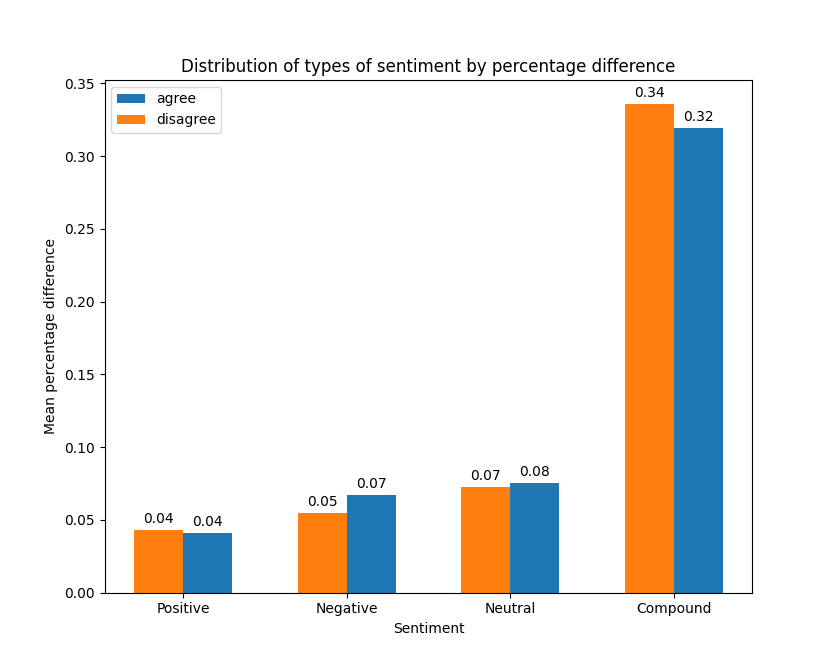
\includegraphics[width=0.8\linewidth]{images/plots/sentiment-analysis.png}
	\caption{Distribution of sentiment types in the FNC-1 dataset}\label{plot:sentiment-analysis}
\end{figure}

\vspace{5mm}

\hspace{-6mm}\begin{minipage}{0.65\linewidth}
VADER produces 3 measures of sentiment - negativity, positivity and neutrality - as well as a compound value of all of them. To visualise the dataset, the percentage difference of the headline and the body text's measures was plotted. The results are shown in figure \ref{plot:sentiment-analysis}. Table \ref{tab:sentiment-sig} shows the results of a significance test; the data had a non-Guassian distribution so a Mann-Whitney U test was used.\\
\end{minipage}
\hspace{5mm}
\begin{minipage}{0.3\linewidth}
\vspace{-12mm}
\begin{tabular}{ll}
\textbf{Sentiment} & \textbf{p-value} \\
Positive           & 0.20988          \\
Negative           & 0.0667           \\
Neutral            & 0.37534          \\
Compound           & 0.08266         
\end{tabular}
\captionof{table}{Sentiment\\analysis significance}
\label{tab:sentiment-sig}
\end{minipage}


No clear trend in the difference between articles that agree and disagree is visible in the plot. Additionally, as none of the p-values is below 0.05, the results lack significance and must be rejected. This quite strongly shows there is no correlation between the difference in the sentiment of headlines and articles, and as a result, sentiment analysis will not provide a meaningful use in the creation of the classifier.

This result is not surprising - the difference between sentiment and congruence was covered in section \ref{lit:sentiment-analysis}. It is possible for two pieces of text to have different sentiments and be in concurrence, or to have similar sentiments and be opposed in meaning, which means sentiment analysis is not suited for this approach.

\subsubsection{Word Vectorisation}
Another approach tested was word vectorisation - codifying a token as a vector comprised of numbers representing a certain quality of the word's meaning, using the context windows discussed in section \ref{lit:word2vec}.

Gensim's Python implementation of word2vec\footnote{\url{https://radimrehurek.com/gensim/models/word2vec.html}} was trained on articles from the raw dataset. As the training data is only used to give word2vec an understanding of how words relate to each other and not used to determine congruence, the data does not need to be labelled. Ten iterations of learning and 250,000 articles were used to train a model with 300 nodes.

The vectorisation model created is of good quality, and able to perform mathematical operations on words, such as the often-used example:

\[\textrm{Woman} + \textrm{King} - \textrm{Man} = \textrm{Queen}\]

With the model trained, it can be used to evaluate the labelled FNC dataset.
For each article in the database, an average vector was calculated for both the headline and the body. This was achieved by summing up each word's vector and dividing by the number of words in the text. The similarity of these vectors was then computed using the \texttt{cosine\_similarites} function in Gensim, which calculates the cosine difference of two vectors. The average difference for both articles that agree and disagree was obtained. The code used to perform this experiment is displayed in appendix \ref{app:vectorisation}.

For articles labelled as agree, the average vector difference was 0.5175, and those labelled disagree had a difference of 0.5050, with a p-value of 0.19308. Like with the sentiment analysis experiment, the lack of significance and the negligible difference between each average shows that this is an ineffective way to determine congruence. This could be because only a few of the words in an article will point to incongruence - by obtaining an average of all of them, the text's meaning will be lost in the noise.

\subsubsection{tf-idf}

\begin{minipage}{0.65\linewidth}
To ascertain the practicality of using tf-idf to detect incongruence, the algorithm set out in section \ref{lit:tfidf} was implemented in Python. To get an informal understanding of the implementation's efficacy, it was used to determine the relevance of a range of keywords to an article about a house fire caused by fireworks. The results are shown in table \ref{tab:tfidf-terms}. As the table shows, the implementation is working as expected - more relevant words, such as 'ablaze', have higher tf-idf values, indicating a higher relevance, and terms such as 'and' and 'football' have a much lower, negligible value.
\\
\end{minipage}
\hspace{5mm}
\begin{minipage}{0.3\linewidth}
\vspace{-2mm}
\begin{tabular}{ll}
\textbf{Term} & \textbf{tf-idf value} \\
ablaze & 421.500 \\
fireworks & 168.600 \\
explosive & 93.667 \\
the & 0.089 \\
and & 0.058 \\
football & 0.000
\end{tabular}
\captionof{table}{tf-idf values for a range of terms}
\label{tab:tfidf-terms}
\end{minipage}

To apply the algorithm to the problem, tf-idf was used to calculate each word's relevance in an article's headline to its body text. A mean was then taken of those values, as shown below. A full code listing is available in the Github repository.\footnote{\url{https://github.com/jacobbarrow/honours/tree/master/experiments/tfidf.py}}

\begin{lstlisting}[language=Python]
for article in articles.values():
    tfidfs = []
    for word in article['headline']:
        tfidfs.append(tfidf(word, article['body'], domain))

    mean = numpy.mean(tfidfs)
\end{lstlisting}

The mean will give an overall relevance between the headline and body of an article. The means were classified according to the article's labelled stance (agree/disagree) and then analysed. For articles labelled as agree, the average tf-idf mean of their headlines was 0.1167. For those labelled disagree, the average was 0.0718. While this difference may initially seem promising, with a p-value of 0.26281, the results must be rejected.

This result is disappointing but expected; tf-idf is used to determine the relevance of a word to a document and does not account for the document's overall sentiment. For instance, consider the following two statements:

\begin{itemize}
	\item Mauve is a trendy colour to paint a house
	\item The worst colour to paint a house is mauve
\end{itemize}

The term 'mauve' appears the same number of times for both of them, so according to tf-idf will have identical relevance. However, each statement's sentiments are opposed, something unable to be determined by just the relevance alone. 

Additionally, using the mean of all headline values may be 'muddying the waters' of the relevancy, as happened in the word vectorisation experiment. However, this may not be as strong a factor, as the difference between a relevant word and an irrelevant word is large, as seen in table \ref{tab:tfidf-terms}, and so would have a more significant effect on the mean.

\section{Analysis and Discussion}
Will talk about results of visualisation here...


\subsection{Classifier}
\subsubsection{Design}
\subsubsection{Implementation}
\pagebreak
\section{Analysis and Discussion}
\pagebreak
\section{Conclusion}
\pagebreak

\bibliographystyle{apacite}
\bibliography{bibliography}

%you can crate this on a extra tex document just like the title or any other part of the document.
\newpage
\begin{appendices}
\iffluff
\section{Project Overview}
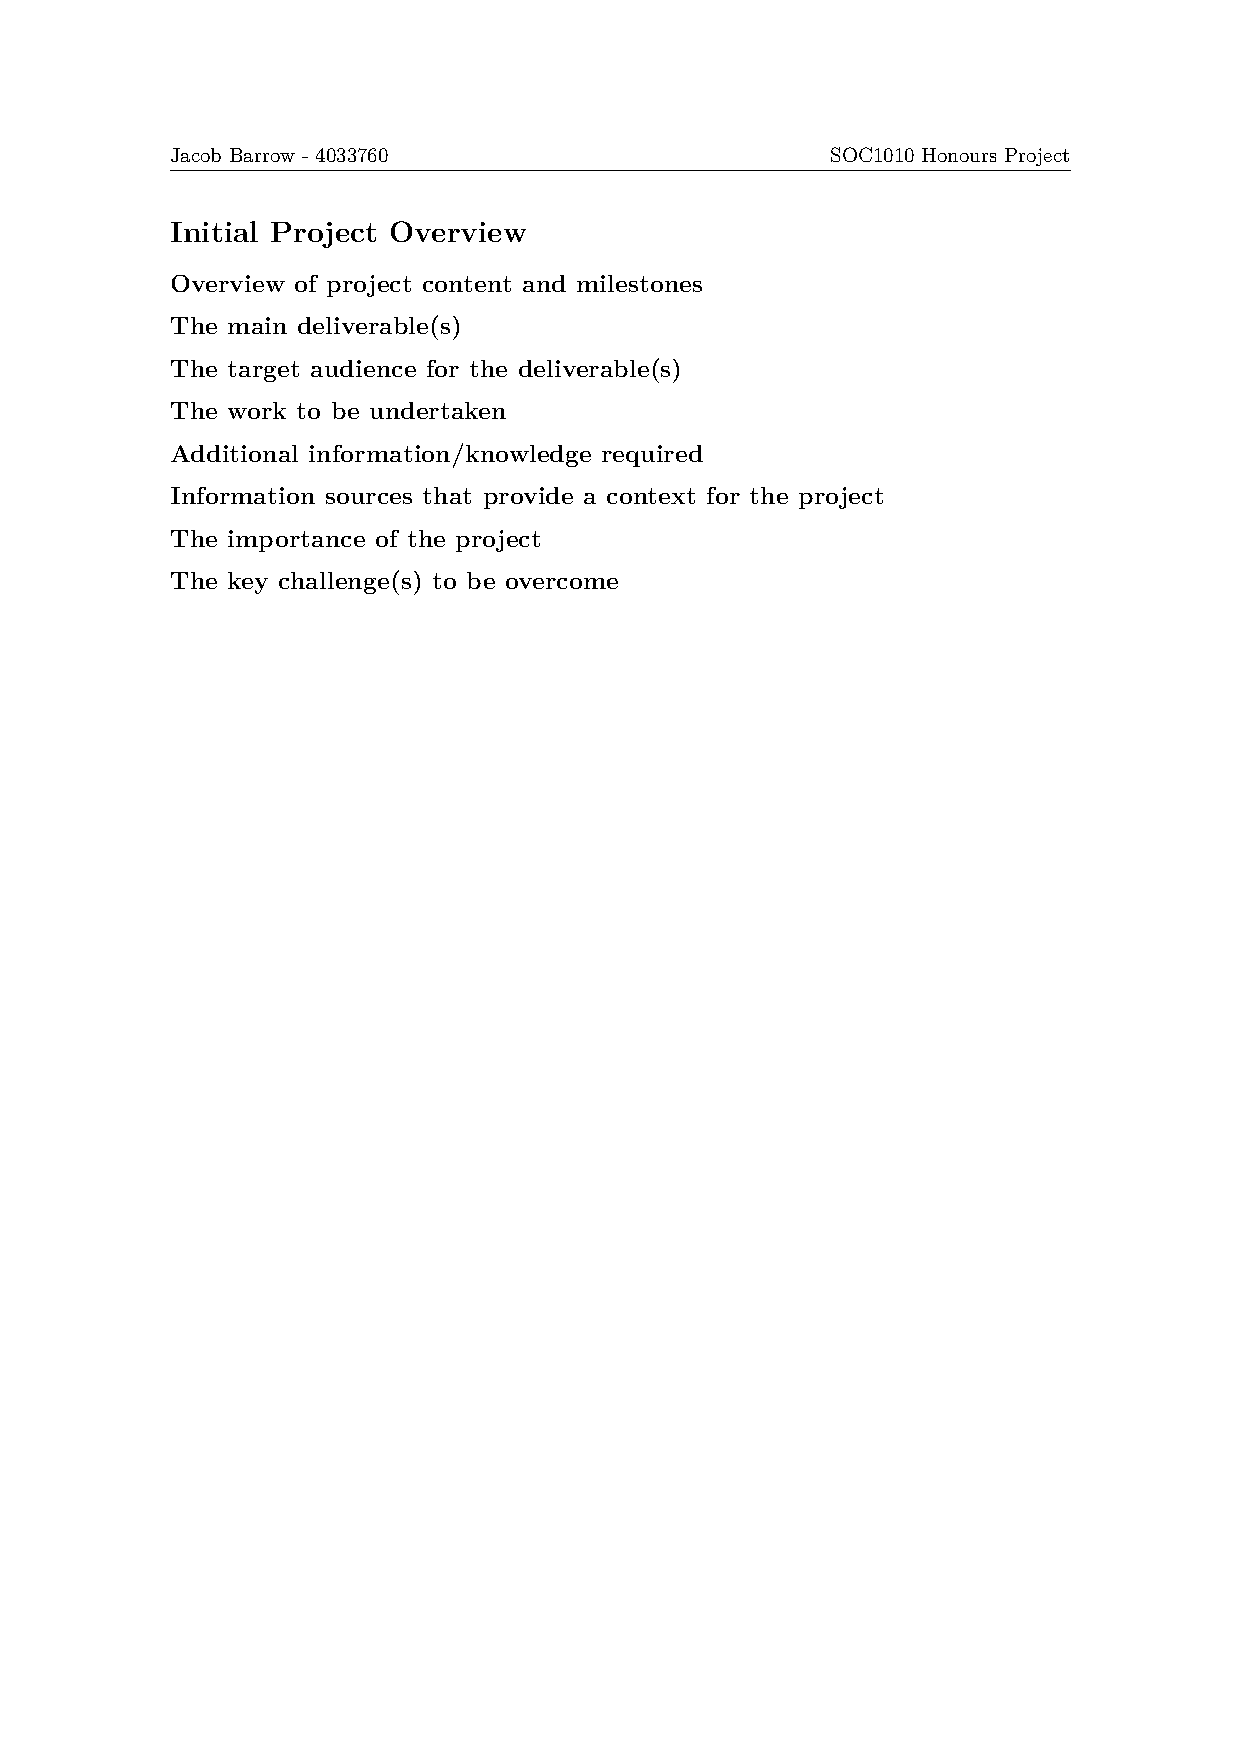
\includepdf[pages=1]{../docs/IPO/IPO}


\section{Second Formal Review Output}
Insert a copy of the project review form you were given at the end of the review by the second marker

\section{Diary Sheets (or other project management evidence)}

\rotatebox{90}{
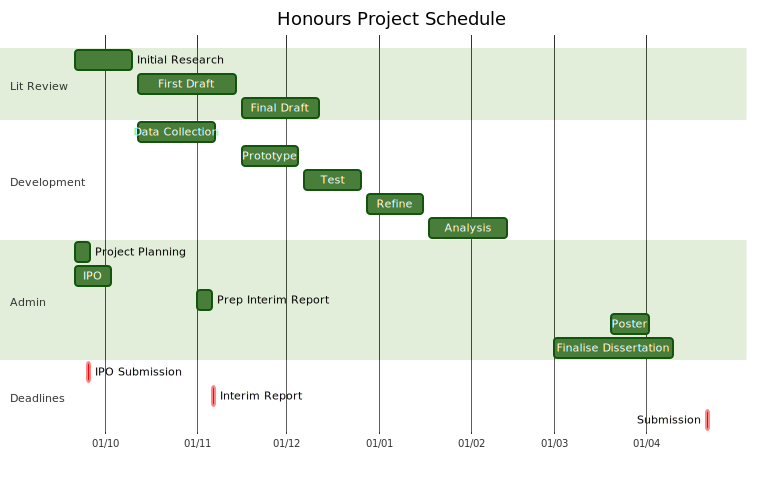
\includegraphics[scale=1,page=1]{../docs/gantt/gantt}
}
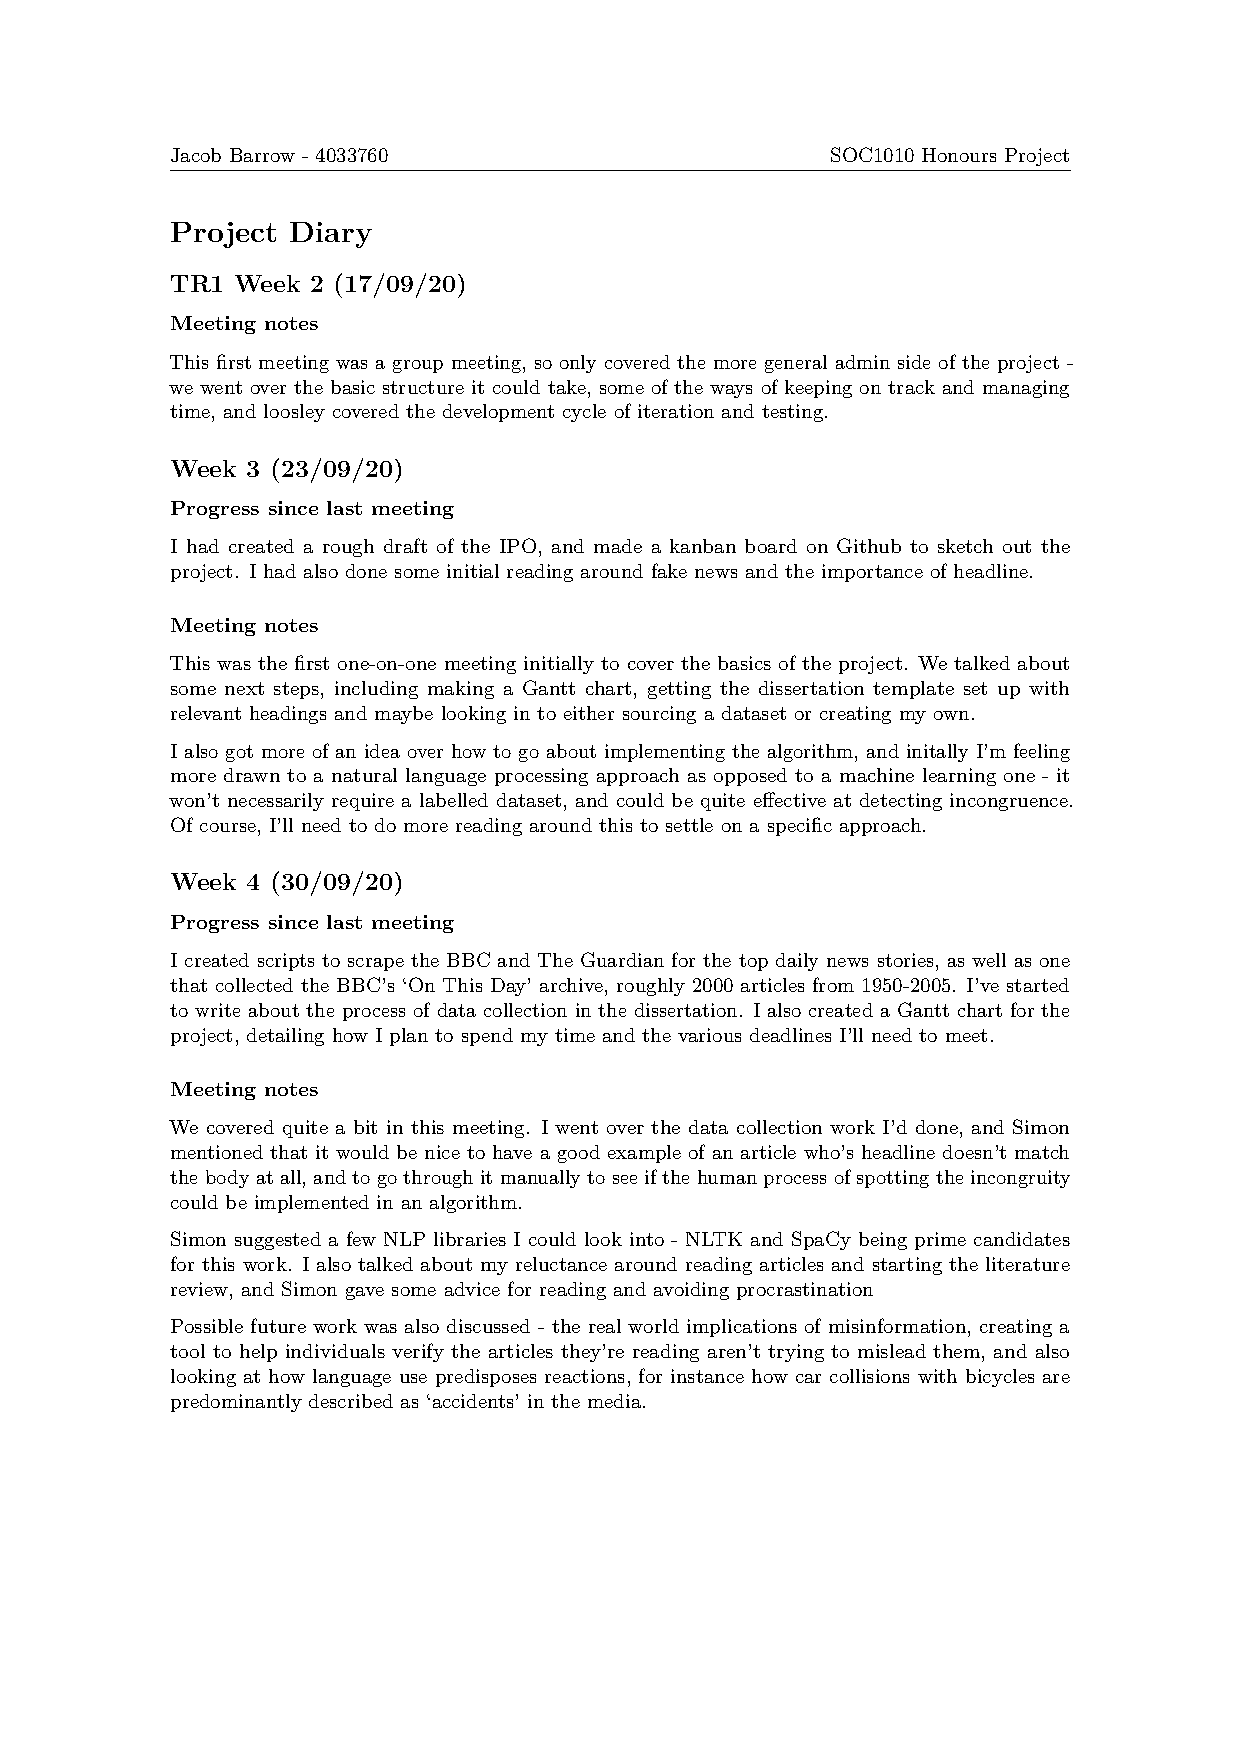
\includepdf[pages=1]{../docs/diary/diary}
\includepdf[pages=2]{../docs/diary/diary}
\includepdf[pages=3]{../docs/diary/diary}
\fi
\section{Data Labelling Ethics}


\begin{subappendices}
\subsection{Participant Information Sheet} \label{app:ethics-participant-info}
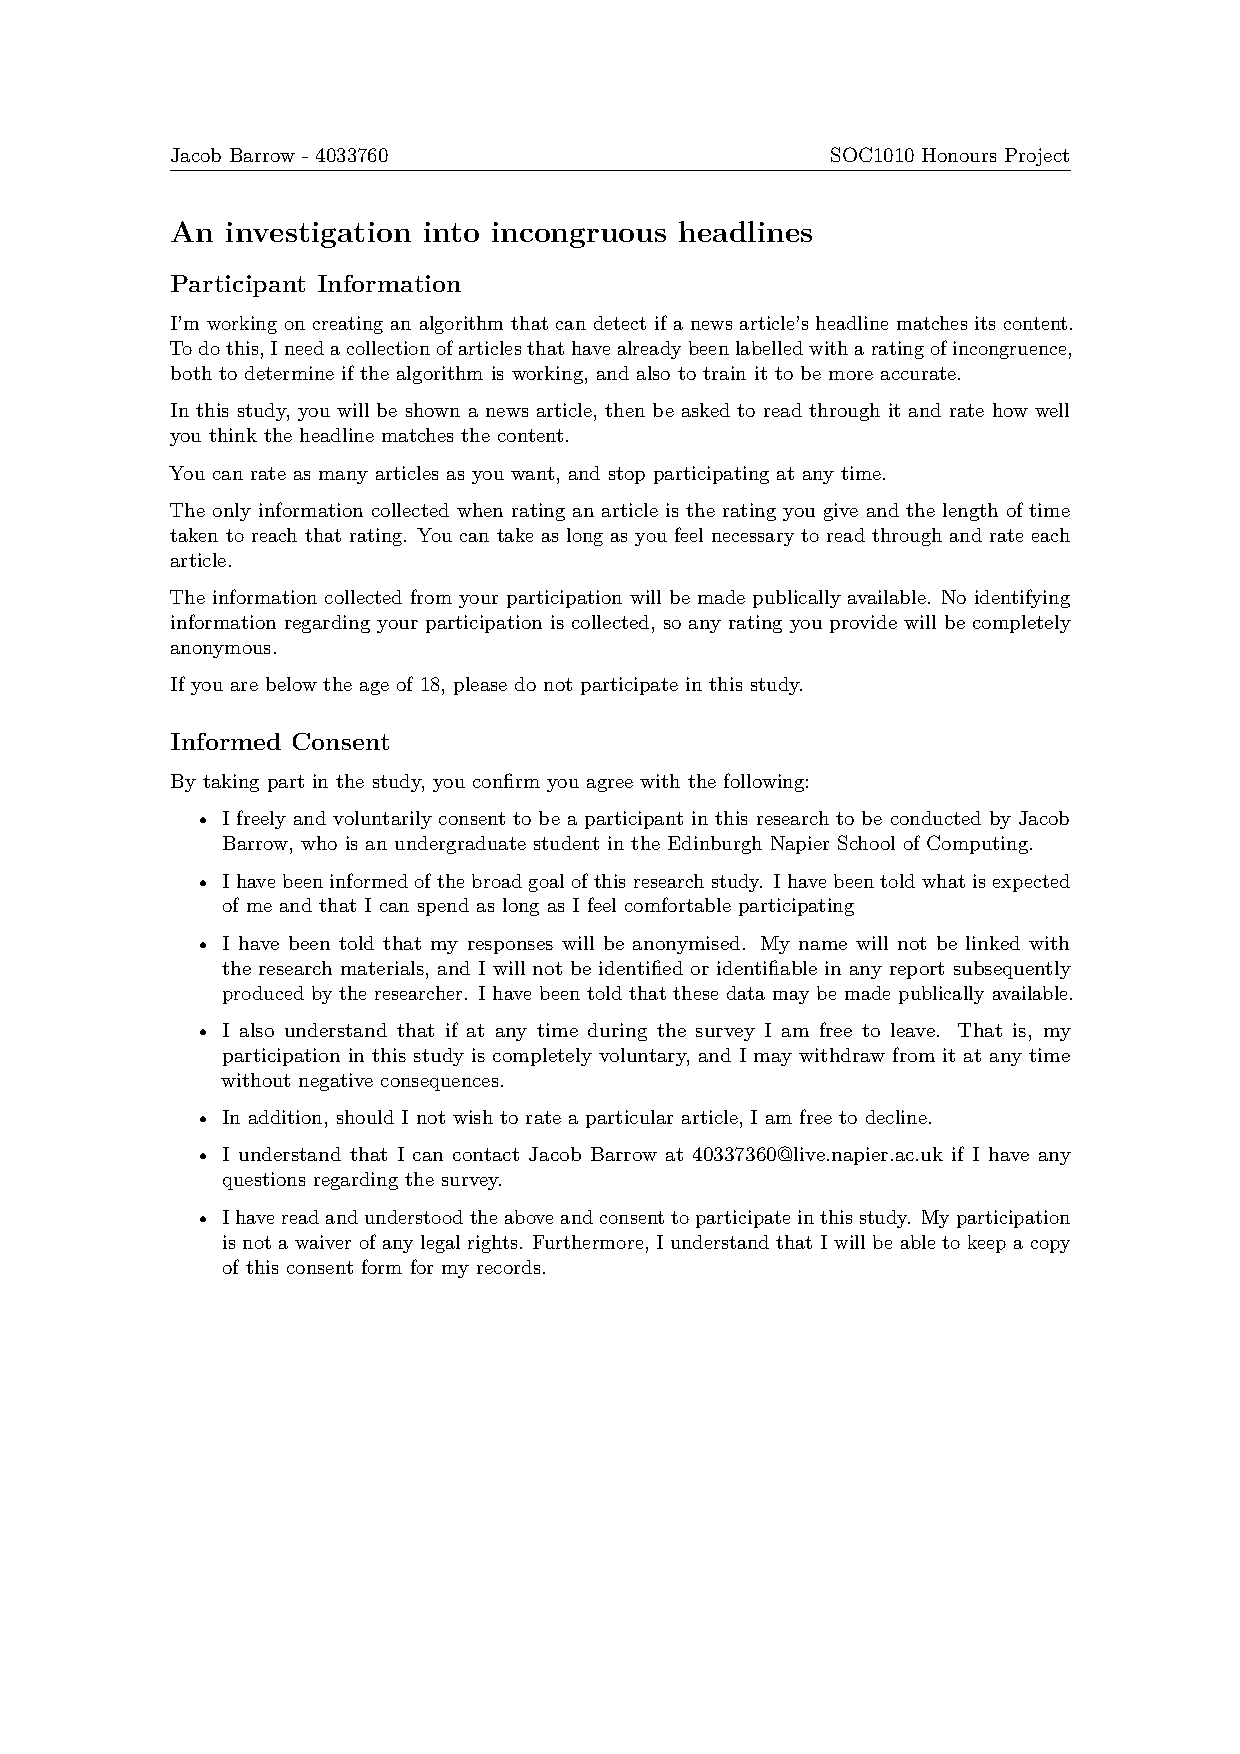
\includepdf[pages=1]{../docs/ethics/participant-info}

\subsection{RI Approval} \label{app:ethics-approval}
\includepdf[pages=1]{../docs/ethics/RI_Approval}
\includepdf[pages=2]{../docs/ethics/RI_Approval}
\includepdf[pages=3]{../docs/ethics/RI_Approval}
\includepdf[pages=4]{../docs/ethics/RI_Approval}
\includepdf[pages=5]{../docs/ethics/RI_Approval}

\subsection{Example Rating Form} \label{app:rating-form}

\includegraphics[scale=0.5]{../docs/ethics/example_rating-just-form}
\end{subappendices}

\section{Code Listings}
\begin{subappendices}
\subsection{Sentiment Analysis Experiment} \label{app:sentiment-analysis}
\lstinputlisting[language=Python]{../experiments/sentiment-analysis.py}

\subsection{Word Vectorisation Experiment} \label{app:vectorisation}
\lstinputlisting[language=Python]{../experiments/vectorisation.py}
\end{subappendices}


\section{Visualiser Wireframe} \label{app:vis-wireframe}
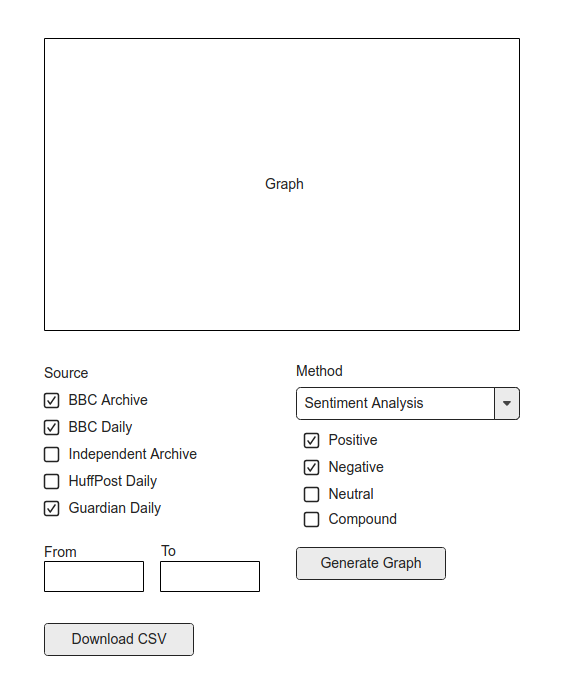
\includegraphics[scale=0.5]{../visualisation/wireframe}

\end{appendices}

\end{document}
